\chapter{Specifikacija programske potpore}
		
	\section{Funkcionalni zahtjevi}
			
			\textit{Navesti \textbf{dionike} koji imaju \textbf{interes u ovom sustavu} ili  \textbf{su nositelji odgovornosti}. To su prije svega korisnici, ali i administratori sustava, naručitelji, razvojni tim.}\\
				
			\textit{Navesti \textbf{aktore} koji izravno \textbf{koriste} ili \textbf{komuniciraju sa sustavom}. Oni mogu imati inicijatorsku ulogu, tj. započinju određene procese u sustavu ili samo sudioničku ulogu, tj. obavljaju određeni posao. Za svakog aktora navesti funkcionalne zahtjeve koji se na njega odnose.}\\
			
			
			\noindent \textbf{Dionici:}
			
			\begin{packed_enum}
				
				\item Neregistrirani korisnik
				\item Registrirani korisnik			
				\item Sklonište za životinje
				\item Razvojni tim
				\item Naručitelji
				
			\end{packed_enum}
			
			\noindent \textbf{Aktori i njihovi funkcionalni zahtjevi:}
			
			
			\begin{packed_enum}
				\item  \underbar{Neregistrirani korisnik (inicijator) može:}
				
				\begin{packed_enum}
					
					\item pregledavati i pretraživati oglašene nestale kućne ljubimce i skloništa za životinje
					\item odabrati nekog od kućnih ljubimaca, čime se otvara mogućnost detaljnijeg pregleda informacija o njemu kao i pregled komunikacije oko potrage za ljubimcem
					\item registrirati se, stvoriti novi korisnički račun za koji su mu potrebni e-pošta, broj telefona, korisničko ime, lozinka te opcionalno (u slučaju registracije kao sklonište) naziv skloništa
					
				\end{packed_enum}
			
				\item  \underbar{Registrirani korisnik (inicijator) može:}
				
				\begin{packed_enum}
					
					\item sve što može neregistrirani korisnik
					\item prijaviti se u sustav
					\item postaviti, izmijeniti i ukloniti oglas o nestalom kućnom ljubimcu
					\item sudjelovati u komunikaciji oko potrage za ljubimcem
					\item pretraživati neaktivne oglase
					
				\end{packed_enum}
			
			\item  \underbar{Sklonište (inicijator) može:}
				
				\begin{packed_enum}
				
					\item sve što može registrirani korisnik
					\item oglašavati pronađene životinje koje se nalazi u prostoru skloništa pomoću kategorije oglasa "\textit{u skloništu}"
					
				\end{packed_enum}
			
			\item  \underbar{Baza podataka (sudionik):}
				
				\begin{packed_enum}
					
					\item pohranjuje sve podatke korisnika
					\item pohranjuje sve podatke vezane uz oglase
					
				\end{packed_enum}
			\end{packed_enum}
			
			\eject 
			
			
				
			\subsection{Obrasci uporabe}
				
				\subsubsection{Opis obrazaca uporabe}

					\noindent \underbar{\textbf{UC1 - Registracija}}
					\begin{packed_item}
	
						\item \textbf{Glavni sudionik:} Neregistrirani korisnik
						\item  \textbf{Cilj:} Stvoriti korisnički račun za pristup sustavu
						\item  \textbf{Sudionici:} Baza podataka
						\item  \textbf{Preduvjet:} -
						\item  \textbf{Opis osnovnog tijeka:}
						
						\item[] \begin{packed_enum}
	
							\item Korisnik odabire opciju za registraciju
							\item Korisnik unosi potrebne korisničke podatke
							\item Korisnik prima obavijest o uspješnoj registraciji
						\end{packed_enum}
						
						\item  \textbf{Opis mogućih odstupanja:}
						
						\item[] \begin{packed_item}
	
							\item[2.a] Odabir već zauzetog korisničkog imena i/ili e-maila, unos korisničkog podatka u nedozvoljenom formatu ili pružanje neispravnog e-maila
							\item[] \begin{packed_enum}
								
								\item Sustav obavještava korisnika o neuspjelom upisu i vraća ga na stranicu za registraciju
								\item Korisnik mijenja potrebne podatke te završava unos ili odustaje od registracije
								
							\end{packed_enum}
							
						\end{packed_item}
					\end{packed_item}
					
					\noindent \underbar{\textbf{UC2 - Prijava u sustav}}
					\begin{packed_item}
	
						\item \textbf{Glavni sudionik:} Neprijavljeni registrirani korisnik
						\item  \textbf{Cilj:} Dobiti pristup mogućnostima registriranih korisnika
						\item  \textbf{Sudionici:} Baza podataka
						\item  \textbf{Preduvjet:} Registracija
						\item  \textbf{Opis osnovnog tijeka:}
						
						\item[] \begin{packed_enum}
	
							\item Unos korisničkog imena i lozinke
							\item Provjera ispravnosti unesenih podataka
							\item Pristup korisničkim funkcijama
						\end{packed_enum}
						
						\item  \textbf{Opis mogućih odstupanja:}
						
						\item[] \begin{packed_item}
	
							\item[2.a] Neispravno korisničko ime/lozinka
							\item[] \begin{packed_enum}
								
								\item Sustav obavještava korisnika o neuspjeloj prijavi i vraća ga na stranicu za prijavu
								
							\end{packed_enum}
							
						\end{packed_item}
					\end{packed_item}
					\pagebreak
					
					\noindent \underbar{\textbf{UC3 - Pregled osobnih podataka}}
					\begin{packed_item}
	
						\item \textbf{Glavni sudionik:} Registrirani korisnik/sklonište za životinje
						\item  \textbf{Cilj:} Pregledati osobne podatke
						\item  \textbf{Sudionici:} Baza podataka
						\item  \textbf{Preduvjet:} Prijava u sustav
						\item  \textbf{Opis osnovnog tijeka:}
						
						\item[] \begin{packed_enum}
	
							\item Korisnik odabire opciju za pregled osobnih podataka
							\item Aplikacija prikazuje osobne podatke korisnika
						\end{packed_enum}
					\end{packed_item}
					
					\noindent \underbar{\textbf{UC4 - Promjena osobnih podataka}}
					\begin{packed_item}
	
						\item \textbf{Glavni sudionik:} Registrirani korisnik/sklonište za životinje
						\item  \textbf{Cilj:} Promjena osobnih podataka
						\item  \textbf{Sudionici:} Baza podataka
						\item  \textbf{Preduvjet:} Prijava u sustav
						\item  \textbf{Opis osnovnog tijeka:}
						
						\item[] \begin{packed_enum}
	
							\item Korisnik pregledava osobne podatke
							\item Korisnik odabire opciju za promjenu osobnih podataka
							\item Korisnik mijenja željene podatke i potvrđuje izmjenu
							\item Baza podataka se ažurira
						\end{packed_enum}
						
						\item \textbf{Opis mogućih odstupanja:} 
						
						
						\item[] \begin{packed_item}
	
							\item[3.a] Korisnik je promijenio svoje podatke, ali ih je zaboravio spremiti
							\item[] \begin{packed_enum}
								
								\item Sustav obavještava korisnika o neuspjeloj promjeni podataka
								\item Korisnik sprema izmijenjene podatke
								
							\end{packed_enum}
					\end{packed_item}
					\end{packed_item}
					
					\noindent \underbar{\textbf{UC5 - Brisanje korisničkog računa}}
					\begin{packed_item}
	
						\item \textbf{Glavni sudionik:} Registrirani korisnik/sklonište za životinje
						\item  \textbf{Cilj:} Brisanje korisničkog računa
						\item  \textbf{Sudionici:} Baza podataka
						\item  \textbf{Preduvjet:} Prijava u sustav
						\item  \textbf{Opis osnovnog tijeka:}
						
						\item[] \begin{packed_enum}
	
							\item Korisnik pregledava osobne podatke
							\item Korisnik odabire opciju za brisanje korisničkog računa
							\item Korisnik potvrđuje odabir
							\item Baza podataka se ažurira
						\end{packed_enum}
					\end{packed_item}
					\pagebreak
					
					\noindent \underbar{\textbf{UC6 - Pretraživanje i pregled oglasa}}
					\begin{packed_item}
	
						\item \textbf{Glavni sudionik:} Korisnik
						\item  \textbf{Cilj:} Pregledati oglase nestalih ljubimaca
						\item  \textbf{Sudionici:} Baza podataka
						\item  \textbf{Preduvjet:} -
						\item  \textbf{Opis osnovnog tijeka:}
						
						\item[] \begin{packed_enum}
	
							\item Korisniku se prikazuju oglasi
							\item Oglasi se mogu filtrirati po relevantnim podacima
							\item Prikaz filtriranih oglasa
						\end{packed_enum}
						
						\item  \textbf{Opis mogućih odstupanja:}
						
						\item[] \begin{packed_item}
	
							\item[2.a] Ne postoji oglas koji odgovara postavljenom filtru
							\item[] \begin{packed_enum}
								
								\item Sustav korisniku prikazuje odgovarajuću poruku
								
							\end{packed_enum}
							
						\end{packed_item}
					\end{packed_item}
					
					\noindent \underbar{\textbf{UC7 - Postavljanje oglasa}}
					\begin{packed_item}
	
						\item \textbf{Glavni sudionik:} Registrirani korisnik
						\item  \textbf{Cilj:} Postaviti oglas o nestalom ljubimcu
						\item  \textbf{Sudionici:} Baza podataka
						\item  \textbf{Preduvjet:} Prijava u sustav
						\item  \textbf{Opis osnovnog tijeka:}
						
						\item[] \begin{packed_enum}
	
							\item Korisnik odabire opciju postavljanja oglasa
							\item Korisnik dobiva mogućnost unošenja sljedećih kategorija podataka o ljubimcu:
								
								\item[] \begin {packed_enum}
									\item vrsta
									\item ime na koje se odaziva
									\item datum i sat nestanka
									\item lokacija nestanka
									\item boja
									\item starost
									\item tekstni opis
									\item do 3 slike
								\end{packed_enum}
							
							\item Ako je korisnik sklonište, postavlja kategoriju oglasa "\textit{u skloništu}"
							\item Korisnik odabire opciju za objavljivanje i njegov oglas postaje vidljiv drugima
						\end{packed_enum}
					\end{packed_item}
					\pagebreak
					
					\noindent \underbar{\textbf{UC8 - Izmjena oglasa}}
					\begin{packed_item}
	
						\item \textbf{Glavni sudionik:} Registrirani korisnik
						\item  \textbf{Cilj:} Izmijeniti oglas o nestalom ljubimcu
						\item  \textbf{Sudionici:} Baza podataka
						\item  \textbf{Preduvjet:} Prijava u sustav
						\item  \textbf{Opis osnovnog tijeka:}
						
						\item[] \begin{packed_enum}
	
							\item Korisnik odabire opciju izmjene svog oglasa
							\item Korisnik mijenja željene podatke, dostupna mu je i promjena kategorije oglasa u neku od sljedećih:
								
								\item[] \begin{packed_enum}
									\item za ljubimcem se traga (\textit{pretpostavljeno})
									\item ljubimac je sretno pronađen
									\item ljubimac nije pronađen, ali se za njim više aktivno ne traga
									\item ljubimac je pronađen uz nesretne okolnosti
								\end{packed_enum}
							\item Korisnik potvrđuje izmjene
						\end{packed_enum}
					\end{packed_item}
					
					\noindent \underbar{\textbf{UC9 - Uklanjanje oglasa}}
					\begin{packed_item}
	
						\item \textbf{Glavni sudionik:} Registrirani korisnik
						\item  \textbf{Cilj:} Ukloniti oglas o nestalom ljubimcu
						\item  \textbf{Sudionici:} Baza podataka
						\item  \textbf{Preduvjet:} Prijava u sustav
						\item  \textbf{Opis osnovnog tijeka:}
						
						\item[] \begin{packed_enum}
	
							\item Korisnik odabire opciju uklanjanja svog oglasa
							\item Uklonjeni oglas i sva pripadna komunikacija nestaje iz popisa vidljivih oglasa, ali se ne briše iz baze podataka
						\end{packed_enum}
					\end{packed_item}
					
					\noindent \underbar{\textbf{UC10 - Oglašavanje u skloništu}}
					\begin{packed_item}
	
						\item \textbf{Glavni sudionik:} Sklonište za životinje
						\item  \textbf{Cilj:} Postaviti oglas o nestalom ljubimcu u skloništu radi pronalaska vlasnika
						\item  \textbf{Sudionici:} Baza podataka
						\item  \textbf{Preduvjet:} Prijava u sustav
						\item  \textbf{Opis osnovnog tijeka:}
						
						\item[] \begin{packed_enum}
	
							\item Sklonište za životinje postavlja oglas kategorije "\textit{u skloništu}"
							\item Oglas se pohranjuje u bazu podataka
							\item Oglas se postavlja na web stranicu i vidljiv je drugim korisnicima
						\end{packed_enum}
					\end{packed_item}
					
					
					
					\noindent \underbar{\textbf{UC11 - Komunikacija}}
					\begin{packed_item}
	
						\item \textbf{Glavni sudionik:} Registrirani korisnik
						\item  \textbf{Cilj:} Sudjelovati u komunikaciji oko potrage za ljubimcem
						\item  \textbf{Sudionici:} Baza podataka
						\item  \textbf{Preduvjet:} Prijava u sustav
						\item  \textbf{Opis osnovnog tijeka:}
						
						\item[] \begin{packed_enum}
	
							\item Korisnik odabire opciju komunikacije
							\item Korisnik unosi poruku koja (uz kontakt podatke korisnika) može sadržavati:
								\item[] \begin{packed_enum}
									\item tekst
									\item sliku
									\item geolokaciju
								\end{packed_enum}
							\item Korisnik potvrđuje poruku koju želi ostaviti na oglasu
							\item Poruka postaje vidljiva ostalim korisnicima
						\end{packed_enum}
					\end{packed_item}
					
					
					
					
					
				\subsubsection{Dijagrami obrazaca uporabe}
					
				\begin{figure}[H]
					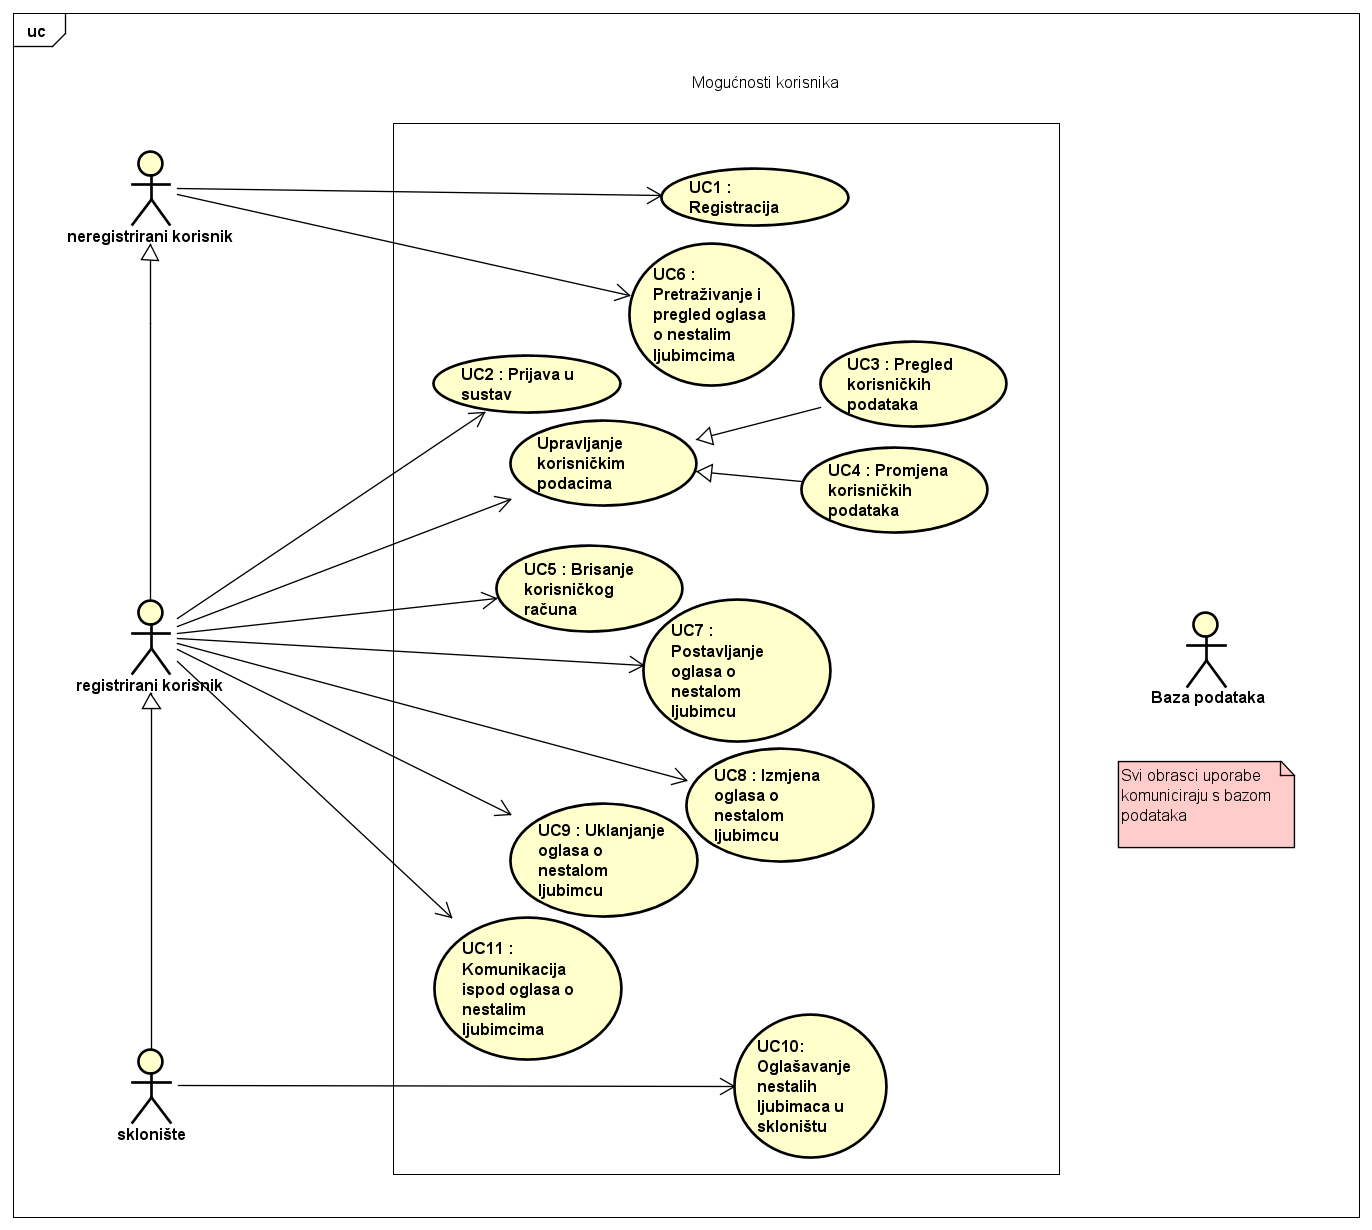
\includegraphics[scale=0.45]{slike/uc_mogucnosti_korisnika.PNG} 
					\centering
					\caption{Dijagram mogućnosti korisnika}
					\label{uc_mogucnosti_korisnika}
				\end{figure}
				
			\subsection{Sekvencijski dijagrami}
				
				\iffalse
				\textit{Nacrtati sekvencijske dijagrame koji modeliraju najvažnije dijelove sustava (max. 4 dijagrama). Ukoliko postoji nedoumica oko odabira, razjasniti s asistentom. Uz svaki dijagram napisati detaljni opis dijagrama.}
				\eject
				\fi
				
			\begin{figure}[H]
				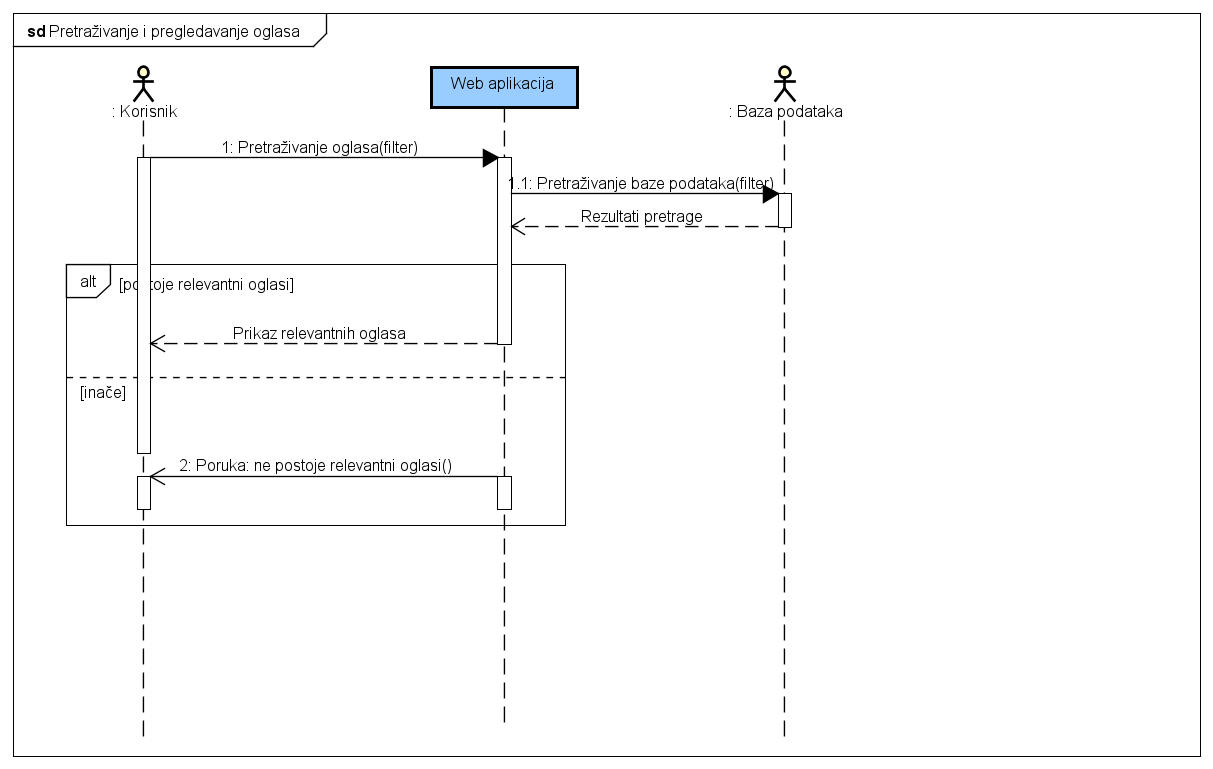
\includegraphics[scale=0.5]{slike/seq_pretrazivanje_pregledavanje_oglasa.PNG} 
				\centering
				\caption{Sekvencijski dijagram pretraživanja i pregledavanja oglasa}
				\label{seq_pretrazivanje_pregledavanje_oglasa}
			\end{figure}
			
			\begin{figure}[H]
				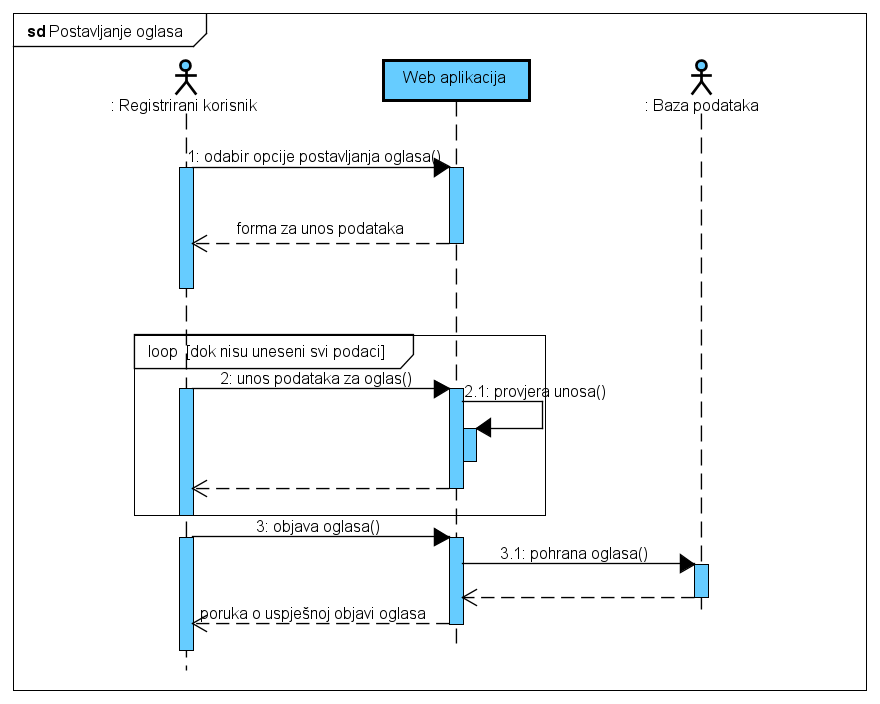
\includegraphics[scale=0.5]{slike/seq_postavljanje_oglasa.PNG} 
				\centering
				\caption{Sekvencijski dijagram postavljanja oglasa}
				\label{seq_postavljanje_oglasa}
			\end{figure}
			
			\begin{figure}[H]
				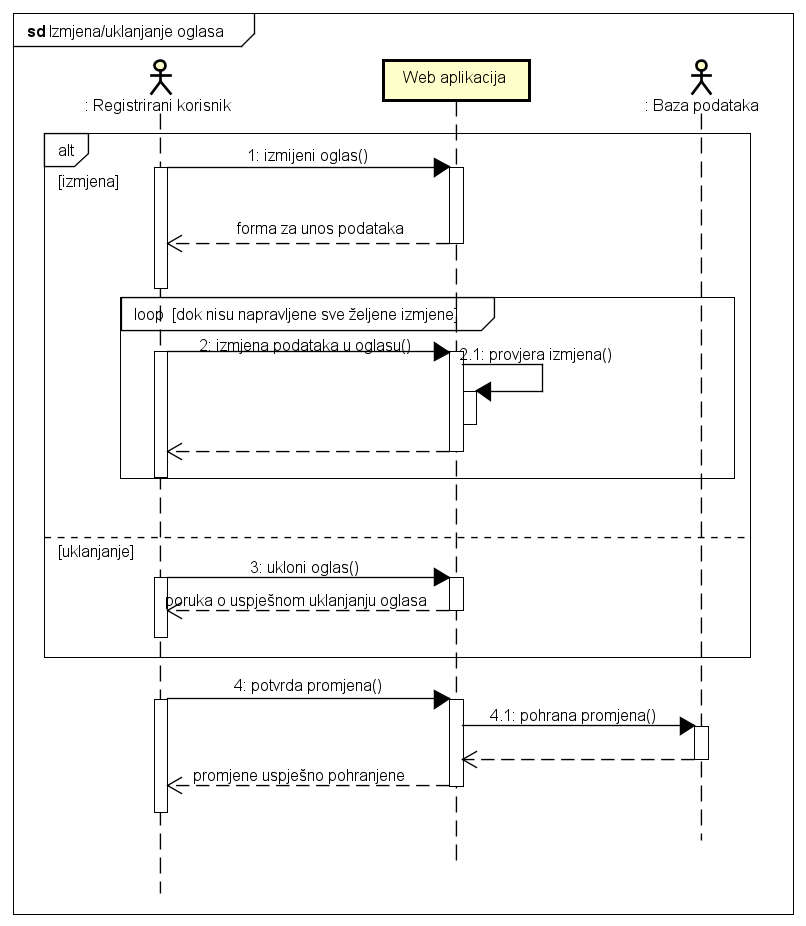
\includegraphics[scale=0.5]{slike/seq_izmjena_oglasa.PNG} 
				\centering
				\caption{Sekvencijski dijagram izmjenjivanja/brisanja oglasa}
				\label{seq_izmjena_oglasa}
			\end{figure}
	
		\section{Ostali zahtjevi}
		 
			 \begin{packed_item}
			 
			 \item Sustav treba omogućiti rad više korisnika u stvarnom vremenu
			 \item Sustav treba funkcionirati ispravno neovisno o web pregledniku ili uređaju
			 \item Korisničko sučelje i sustav moraju podržavati hrvatsku abecedu (dijakritičke znakove) pri unosu i prikazu tekstualnog sadržaja
			 \item Učitavanje početne stranice ne smije trajati duže od nekoliko sekundi
			 \item Izvršavanje dijela programa u kojem se pristupa bazi podataka ne smije trajati duže od nekoliko sekundi
			 \item Sustav treba biti implementiran kao web aplikacija koristeći objektno-orijentirane jezike
			 \item Neispravno korištenje korisničkog sučelja ne smije narušiti funkcionalnost i rad sustava
			 \item Nadogradnja sustava ne smije narušavati postojeće funkcionalnosti sustava
			 \item Sustav treba biti jednostavan za korištenje, korisnici se moraju znati koristiti sučeljem bez opširnih uputa
			 \item Veza s bazom mora biti kvalitetno zaštićena, brza i otporna na vanjske greške
			 \item Pristup sustavu mora biti omogućen iz javne mreže pomoću HTTPS
			 
			 
			 \end{packed_item}
			 
			 
			 
	